
%% Template Elsevier for Neuroimage

%% Use the option review to obtain double line spacing
%\documentclass[authoryear,preprint,review]{elsarticle}
\documentclass[authoryear]{elsarticle}
%\usepackage[framed,numbered,autolinebreaks,useliterate]{mcode}
\usepackage[framed,autolinebreaks,useliterate]{mcode}
\usepackage{natbib}
\usepackage{amsmath}
%\usepackage{lineno}
\usepackage{rotating}

\usepackage{hyperref}
\usepackage{amssymb}
\usepackage{amsfonts}


%\usepackage{algorithm2e}
%\usepackage{algorithmic}
%\usepackage{todonotes}
\usepackage{pdflscape}
\journal{Neuroimage}
\usepackage{color,transparent}
%\usepackage{color} 
%\pdfoptionpdfminorversion 6
\pdfminorversion=5

%\usepackage{graphicx}
%\usepackage{subcaption}
%\usepackage{mwe}
\usepackage{subfig}
\usepackage{caption}
%\usepackage{subcaption}
\usepackage{setspace}

\begin{document}

% Title must be 150 words or less
\begin{frontmatter}
%\title{Feasibility of multi-centric fMRI connectivity studies of Alzheimer's disease}
%\title{Feasibility of multi-centric fMRI connectivity and impact }

%\title{Measurement bias and statistical power in multi-centric resting-state fMRI connectivity}
\title{Statistical power and measurement bias in multi-centric resting-state fMRI connectivity}


%\title{A power analysis for multisite studies in resting-state functional connectivity, with an application to clinical trials in Alzheimer's disease}

\author[a,b]{Christian~Dansereau}
\author[c]{Celine~Risterucci}
\author[c]{Emilio~Merlo Pich}
\author[a]{Yassine~Benhajali}
\author[a]{Pierre~Orban}
\author[d]{Douglas~Arnold}
\author[a,b]{Pierre~Bellec\corref{cor1}}
\ead{pierre.bellec@criugm.qc.ca}
\cortext[cor1]{Corresponding author}
\address[a]{Centre de Recherche de l'Institut Universitaire de G\'eriatrie de Montr\'eal, Montr\'eal, CA}
\address[b]{D\'epartement d'Informatique et de recherche op\'erationnelle, Universit\'e de Montr\'eal, Montr\'eal,CA}
\address[c]{F. Hoffmann-La Roche Ldt., Basel, Switzerland}
\address[d]{NeuroRx, Montreal, Quebec, Canada}

% Please keep the abstract between 250 and 300 words
\begin{abstract}


\end{abstract}

%-- 
\begin{keyword}
multisite \sep multiprotocol \sep bias \sep statistical power \sep sample size \sep resting-state \sep fMRI, connectivity
%fmri \sep effect size \sep multisite \sep clinical trial \sep AD biomarker
\end{keyword}
\end{frontmatter}

% Unique number for each line
%\linenumbers
%\listoftodos

\section*{Highlights}

\begin{itemize}
\item etc
 %\item The impact of the number of nodes, or scale, on the sensitivity of a connectome-wide association study is systematically evaluated.
 %\item A procedure is presented that controls the false-discovery rate within- and between scales.
 %\item The technique is evaluated on a simulation of multiscale changes in connectome organization.
 %\item The technique is applied on three different datasets, for which there is a good a priori knowledge on the underlying connectivity changes.
 %\item Several recent procedures for connectome-wide association are compared.
\end{itemize}

\section{Introduction}

% Magic paragraph
\paragraph{Main objective}
Studies collecting brain images at multiple sites are becoming increasingly common in resting-state functional magnetic resonance imaging (rs-fMRI). In particular, some consortia have retrospectively shared rs-fMRI data from multiple independent studies of comparable populations, with the objective of dramatically increasing the sample size at the cost of decreased sample homogeneity, e.g. normal controls in the 1000 functional connectome project (FCP) \citep{Biswal2010}, children and adolescents suffering from attention deficit hyperactivity disorder from the ADHD200 \citep{ADHD200,Fair2012}, or individual diagnosed with autism spectrum disorder in ABIDE \citep{Nielsen2013}. Recruitment of patient populations in a limited time frame may also require acquisitions at multiple sites, e.g. the Alzheimer’s disease neuroimaging initiative (ADNI) \citep{Mueller2005} (REF2) fBIRN \citep{Friedman2006,Friedman2006a}, which is a common practice in pharmaceutical clinical trials at phase II and III \footnote{\url{http://www.roche-trials.com/trialDetailsGet.action?studyNumber=BP28248}}. An important benefit of multisite acquisitions is to offer improved generalization compared to single site studies, due to more diversity in scanners and populations. These additional sources of variance may however decrease the statistical power, and somewhat mitigate the benefits of having a large sample size. In this work, our main objective was to quantitatively assess the impact of inter-site variability on statistical power, for rs-fMRI group comparison.

\paragraph{Statistical power}
A simple and popular measure of individual resting-state connectivity is the Pearson’s correlation coefficient between the average temporal rs-fMRI fluctuations of two brain parcels. To compare two groups, a general linear model (GLM) is typically used to establish statistical difference in average connectivity between the groups, while accounting for possible confounding variables such as age, sex or the amount of head motion during the scan. Based on the parameters estimated by the GLM, a p-value is generated for each connection to quantify the probability that the difference in average connectivity is significantly distant from zero \citep{Worsley1995}. If the estimated p-value is smaller than a prescribed false-positive rate, say $\alpha=0.05$, then the difference in connectivity is deemed significant. Although in classical statistical testing the statistical decision is made purely based on the p-value, or type I errors, the statistical power is as critical as it controls for type II errors, i.e. failing to detect true differences. The statistical power is defined as the probability of finding a significant difference, when there is indeed a true difference. In the GLM, the statistical power in addition to sample size \citep{Desmond2002}: (1) the sample size; (2) the absolute size of the effect, i.e. the difference in mean connectivity between groups; and, (3) the variability of measures. 
The careful design of a study typically involves selecting the sample size in order to achieve a reasonable statistical power, say larger than $80\%$. But the choice of a multisite vs monosite study design may also impact statistical power by increasing the variability of measures. The recent work of \cite{Yang2014} have shown the presence of a significant bias in rs-fMRI measures between site, yet, to the best of our knowledge, the amplitude of this bias and its implications for statistical power calculation are not currently documented in the literature. 

\paragraph{Sources of variance in rs-fMRI}
The variability of rs-fMRI connectivity measures has both physiological and instrumental origins. Some sources of variability are shared by monosite and multisite studies, while others are specific of multisite studies. We can first note that rs-fMRI connectivity only has moderate-to-good test-rest reliability, when the measure is repeated for the same subjects in the same scanner \citep{Shehzad2009}. Many physiological factors likely contribute to these variations, such as the cognitive state of the subject, the level of alertness/drowsiness, circadian rhythm, hunger, medical regimen, potential neurostimulants, amongst others. There is also an instrumental variability even within subject and within scanner. The thermal noise in rs-fMRI only has a small amplitude (REF), but there are non-uniformity artefacts which have a strong impact on the signal, and will vary from session to session with the positioning of subjects as well as the adjustment of shimming (REF). Another source of within-site variations is the difference in connectivity across subjects. These variations are substantial and have been associated to a myriad of variables and clinical conditions (REF review). Taken together, the combination of within- and between-subjects variance is expected to have a large amplitude even at a single site. Multisite studies will add additional sources of physiological variations, as populations at different sites may substantially differ in terms of ethnicity, language, diet, socioeconomic status, exposure to pollutants, typical medication, quality of health services, etc. Some of these factors will be present even if stringent and harmonized inclusion/exclusion criteria are applied, e.g. diet or language. In terms of instrumentation, the fMRI measurements across sites can be affected by the scanner make and model \citep{Friedman2006}, sequence parameters such as repetition time, flip angle, or acquisition volume \citep{Friedman2006a}, experimental design such as eyes-open/eyes-closed \citep{Yan2009} or experiment duration \citep{VanDijk2010}, and scanning environment such as sound attenuation measures \citep{Elliott1999}, room temperature \citep{Vanhoutte2006}, or head-motion restraint techniques \citep{Edward2000}. Many of these parameters can be harmonized to some extent, but some differences may always remain, e.g. even identical scanners may have different software versions or upgrades.

\paragraph{Specific objectives}
To establish the impact of multisite acquisitions on statistical power in rs-fMRI, we first specifically aimed at characterizing the amplitude of the inter-site bias in real rs-fMRI measures, relative to intra-site variance. We based our evaluation on N=345 young healthy participants from the 1000 Functional Connectomes Project (FCP), including rs-fMRI samples independently collected at 8 imaging sites with 3T scanners in Germany, the United Kingdom, Australia and the United States of America. Datasets in this study were shared retrospectively and every documented parameters of image acquisition varied across studies. This data sample thus represents a worst-case-scenario in terms of 3T instrumental inter-site variations. Our second specific aim was to evaluate the impact of such inter-site bias on the detection power of rs-fMRI group comparison, in relation with sample size, group balancing and interaction between sites and group differences. We implemented for this purpose a series of simulation, mixing synthetic data with real data from the 1000 FCP. One of the particularity of the 1000 FCP is the presence of one large site of $\sim200$ subjects and 7 small sites of $\sim20$ subjects per site. We were therefore able to implement realistic scenarios following either a monosite or a multisite design, with the same total sample size.

\section{Method}


\subsection{Data samples}

\paragraph{Participants}
The paper studies 345 cognitively normal young adults (CNY) from a subset of subjects from the 1000 functional connectome project\footnote{\url{http://fcon_1000.projects.nitrc.org/}}. Only 3 tesla scanners from the following geographical locations: Germany, the United Kingdom, Australia and the United States of America were used, with a minimum of 15 subjects / site, including male and female representation. The sample was restricted to sites with full brain coverage in term of their field of view and a minimum of 50 functional volumes / run after high-motion censoring. From the 345 subjects (150 males, age range = 18-46 years) the total time of acquisition ranged between 6 and 7.5 min / run. The average age of the pooled dataset is 23.8 $\pm$5.14 years old with a male ratio of 41\% across all sites, see Table \ref{table_dataset} for more details on each site selected in the study. The experimental protocols for all datasets were approved by their respective ethic boards.  

\begin{table}[tbp]
\resizebox{\columnwidth}{!}{%
\begin{tabular}{lllllllllll}
\textbf{Site}         & \textbf{Magnet} & \textbf{Scanner make} & \textbf{Channels} & \textbf{N} & \textbf{N final} & \textbf{Sex} & \textbf{Age} & \textbf{TR} & \textbf{\# Slices} & \textbf{\# Frames} \\
\hline
Baltimore, USA        & 3T              & N/A                   & N/A               & 23   & 21         & 8M/15F       & 20-40        & 2.5         & 47                 & 123                \\
Berlin, Germany       & 3T              & Siemens Tim Trio      & 12                & 26   & 26         & 13M/13F      & 23-44        & 2.3         & 34                 & 195                \\
Cambridge, USA        & 3T              & Siemens Tim Trio      & 12                & 198  & 195        & 75M/123F     & 18-30        & 3           & 47                 & 119                \\
Newark, USA           & 3T              & N/A                   & N/A               & 19   & 17         & 9M/10F       & 21-39        & 2           & 32                 & 135                \\
NewYork\_b, USA       & 3T              & Siemens               & N/A               & 20   & 18         & 8M/12F       & 18-46        & 2           & 33                 & 175                \\
Oxford, UK            & 3T              & Siemens Tim Trio      & 12                & 22   & 20         & 12M/10F      & 20-35        & 2           & 34                 & 175                \\
Queensland, Australia & 4T              & Bruker                & 1                 & 19   & 17         & 11M/8F       & 20-34        & 2.1         & 36                 & 190                \\
SaintLouis, USA       & 3T              & Siemens Tim Trio      & 12                & 31   & 31         & 14M/17F      & 21-29        & 2.5         & 32                 & 127              
\end{tabular}
}
\caption{Sites selected from the 1000 Functional Connectome Project.}
\label{table_dataset}
\end{table}

\subsection{Computational environment}
All experiments were performed using the NeuroImaging Analysis Kit (NIAK\footnote{\url{http://simexp.github.io/niak/}} ) (Bellec et al., 2011) version 0.12.18, under CentOS version 6.3 with Octave\footnote{\url{http://gnu.octave.org/}} version 3.8.1 and the Minc toolkit\footnote{\url{http://www.bic.mni.mcgill.ca/ServicesSoftware/ServicesSoftwareMincToolKit}} version 0.3.18. Analyses were executed in parallel on the ”Mammouth” supercomputer\footnote{\url{http://www.calculquebec.ca/index.php/en/resources/compute-servers/mammouth-serie-ii}} , using the pipeline system for Octave and Matlab \citep{Bellec2012}, version 1.0.2. The scripts used for processing can be found on Github\footnote{\url{http://www.calculquebec.ca/index.php/en/resources/compute-servers/mammouth-serie-ii}}. For visualization Python 2.7.9 from the Anaconda 2.2.0\footnote{\url{http://docs.continuum.io/anaconda/index}} distribution were used along with Matplotlib\footnote{\url{http://matplotlib.org/}} \citep{matplotlib}, Seaborn\footnote{\url{http://stanford.edu/~mwaskom/software/seaborn/index.html}} and Nilearn\footnote{\url{http://nilearn.github.io/}} for brain map visualizations.


\subsection{Preprocessing}
Each fMRI dataset was corrected for slice timing; a rigid-body motion was then estimated for each time frame, both within and between runs, as well as between one fMRI run and the T1 scan for each subject \citep{Collins1994}. The T1 scan was itself non-linearly co-registered to the Montreal Neurological Institute (MNI) ICBM152 stereotaxic symmetric template \citep{Fonov2011}, using the CIVET pipeline \citep{Ad-Dab'bagh2006}. The rigid-body, fMRI-to-T1 and T1-to-stereotaxic transformations were all combined to resample the fMRI in MNI space at a 3 mm isotropic resolution. To minimize artifacts due to excessive motion, all time frames showing a displacement greater than 0.5 mm were removed \citep{Power2012}. A minimum of 50 unscrubbed volumes per run was required for further analysis (13 subjects were rejected). The following nuisance covariates were regressed out from fMRI time series: slow time drifts (basis of discrete cosines with a 0.01 Hz highpass cut-off), average signals in conservative masks of the white matter and the lateral ventricles as well as the first principal components (accounting for 95\% variance) of the six rigid-body motion parameters and their squares \citep{Giove2009,Lund2006}. The fMRI volumes were finally spatially smoothed with a 6 mm isotropic Gaussian blurring kernel. A more detailed description of the pipeline can be found on the NIAK website\footnote{\url{http://niak.simexp-lab.org/pipe_preprocessing.html}} and Github\footnote{\url{https://github.com/SIMEXP/multisite}}.

\subsection{Inter-site bias in resting-state connectivity}
We first compared the functional connectivity measures derived from different sites of the 1000 FCP. The connectivity measures were obtained from the Pearson’s correlation coefficient between the average temporal rs-fMRI fluctuations of a given pair of brain parcels. $R=100$ parcels were obtained from a brain parcellation described in \cite{Orban2015}, and generated using a bootstrap analysis of stable clusters \citep{Bellec2010c} from the Cambridge cohort of the 1000 FCP. For each subject, a $100 \times 100$ functional connectome matrix was generated including all parcel-to-parcel connections. 

To quantify the inter-site bias we proposed to calculate the difference between the intra-site variability and the inter-site variability, we first obtained the intra-site variance for each site by computing the standard deviation (STD) distribution across-connections. In a second step we obtained the inter-site variance distribution by computing the STD across-site for each average connection of the connectivity matrix.

In order to quantify if the functional connectivity differences were significative between sites, we used a  general linear model (GLM). The age, sex and frame displacement (FD) confounding variables were included in the model.  The variables were corrected to have a zero mean across subjects, and an intercept (i.e. a column filled with 1) was added to capture the inter-site global average. A p-value was generated for each connection to quantify the probability that the difference in average connectivity was significantly distant from zero \citep{Worsley1995}. The number of false discovery was also controlled ($\alpha=0.05$) using a Benjamini–Hochberg false discovery rate (FDR) procedure \citep{Benjamini1995}.


\subsection{Simulations}
\paragraph{Data generation process}

We implemented Monte-Carlo simulations based on the 1000 FCP sample, with 8 sites for a total of 345 subjects. The multisite simulations were based on 7 sites, totaling 150 subjects, and the monosite simulations were based on the Cambridge site, with 195 subjects. The following data generation model was used to simulate tests of group difference. A subsample of subjects of fixed size was first selected randomly at each site. For each site, a ratio $W$ of the selected subjects were randomly assigned to a 'treatment' group. For the subjects in the treatment group, a fixed value was added to achieve a given relative effect size (Cohen's $d$, see Section below) to 11 connections, previously described in \cite{Orban2015}. \cite{Orban2015} first selected from a literature review the pairs of regions believed to be affected in Alzheimer disease progression due to their difference in connectivity between cognitively normal subjects and patient with dementia of the Alzheimer type. Second, from that selection a subset of candidate pairs was retained based on their reproducibility score at a test-retest experiment conducted using the NYU TRT dataset \citep{Zuo2010} (a dataset where each subject is scan 3 times, across 3 sessions).  

In summary, the simulations had the following parameters:

\begin{itemize}
 \item $W$: The allocation ratio of participants,
 \item $d$ effect size (Cohen’s $d$),
 \item $di=0.5$ interaction site-pathology effect,
 \item $B=10^3$ number of simulations,
 \item $s$ average standard deviation from the reference dataset,
 \item $\alpha=0.001$ threshold of false-positive rate,
\end{itemize}

%The detection power quantitatively express the reproducibility of the findings and we can therefore choose a sample size to achieve the desired detection power for a given probability of rejecting the null hypothesis $alpha$.

\paragraph{Effect size (Cohen's $d$)}
The normalized Cohen's $d$ was used to estimate the effect size and it is defined as the difference between two means $\bar{x_{1}},\bar{x_{2}}$ divided by a standard deviation from the data $s$.

For each site an effect is added to the connectivity of $W$ of the subjects, selected randomly ("pathological" group):
\begin{equation}
	y_{i,j} = y_{i,j} + \mu.
\end{equation}

The parameter $\mu$ is chosen to obtain a particular effect size (expressed as the $d$ of Cohen)
\begin{equation}
\label{eq_cohen}
   \begin{array}{l l}
     d = \frac{\mu}{s_{i,j}},     
   \end{array}
\end{equation}
where $s_{i,j}$ is the standard deviation between region $i$ and $j$ for the reference population (mono-site). 

In order to introduce the same effect-size across the monosite and multisite datasets we are taking the standard deviation from the previously mentioned Cambridge cohort as the reference.  The connection $y_{i,j}$ of the randomly affected subjects ("treatment" group) are therefore calculated $y_{i,j} = y_{i,j} + d\times s_{i,j}$.

\paragraph{GLM model}
In order to detect changes on each connection pair between the artificially created groups, a general linear model (GLM) was applied and the following confounding variables were modelled in the analysis: age, sex and frame displacement (FD). To account for site-specific bias $S-1$ dummy-variables (binary vectors $1\times S$) were added to the model with $S$ being the total number of sites used in the study. The variables are corrected to have a zero mean across subjects, and an intercept (i.e. a column filled with 1) is added to $\mathbf{X}$ to capture the global average. The GLM relies on the following stochastic model Equation\ref{eq_glm_dummy}.

\begin{equation}
\label{eq_glm_dummy}
 \mathbf{Y} = \mathbf{X}\mathbf{\beta} + \mathbf{V}\mathbf{\gamma}+ \mathbf{E},
\end{equation}
\begin{itemize}
 \item $\mathbf{Y}$: $N\times 1$, connectivity value for the pair ($i,j$),
 \item $\mathbf{X}$: $N\times K$, explainable variables,
 \item $\mathbf{\beta}$: $1 \times K$, regression values for each explainable variable,
 \item $\mathbf{V}$: $N\times S$, each column code for a site (0/1),
 \item $\mathbf{\gamma}$: $1\times S$, site average connectivity,
 \item $\mathbf{E}$: $N\times 1$, residual values from the regression,
\end{itemize}
with $N$ the number of subjects, $K$ the number of explainable variables and $S$ the number of sites. Where $\mathbf{\beta}$ is an unknown $1\times K$ vector of linear regression coefficients, $\mathbf{\gamma}$ is a $1\times S$ vector of linear regression coefficients representing the contribution of each site and $\mathbf{E}$ is a $N\times 1$ random (noise) multivariate Gaussian variable. As data generated from different subjects are statistically independent, and under an homoscedasticity assumption, the regression coefficients $\mathbf{\beta}$ can be estimated with ordinary least squares.

% statistical detection and sensitivity
\paragraph{Statistical detection and sensitivity}
We relied on the following parametric assumptions on the noise $\mathbf{E}$ (1) that its rows are independent; (2) that each element follows a normal distribution with zero mean, and (3) that the variance of all elements are constant within a column, also called the homoscedasticity assumptions. As the data generated from different subjects are statistically independent the first assumption is reasonable. We tested the normality and homoscedasticity assumptions on real datasets. Under these parametric assumptions, the regression coefficients $\mathbf{\beta}$ and $\mathbf{\gamma}$ can be estimated with ordinary least squares and, for a given “contrast” (difference between the control and 'treatment' group) the significance of the contrast is assessed by a Student $t$-test.

The sensitivity of the test was evaluated by the average detection performance of all the samples (see Equation \ref{eq_sensitivity}). For each sample $b$, we have a $p$-value $p^{*}_b$ and the detection sensitivity is estimated by the probability of $p^{*}_b$ being inferior or equal to $\alpha=0.001$.

\begin{equation}
   \frac{1}{B}\sum\limits_{b=1}^B\left(p^{*}_b\leq0.001\right).
   \label{eq_sensitivity}
\end{equation}

%Using sub-sampling it is possible to obtain an estimate of the mean statistical power over all samples which is call the detection power. These parameter estimates can then be used in simulation experiments to generate power curves.

% The simulation scenarios
\paragraph{Simulation scenarios}
For each experiment using real data, all effect size in the range 0 to 2 Cohen’s $d$ with a step of 0.01 were considered. For each experiment we performed $B=10^3$ simulations using 80\% subsampling and the reported allocation ratio of participants $W$ and its inverse $1-W$ was attributed randomly to the treatment population for each site. We implemented the following experiments:

\begin{itemize}
 \item We first checked how the total number of subject impact sensitivity using 3 different sample size (40, 80, 120) for an allocation ratio of $W=0.5$,
 \item We then checked how the allocation ratio of participants $W$ impact sensitivity using 3 different ratio ($W=0.5,0.3,0.15$) for a total sample size of 120,
 \item Including an interaction site-pathology effect of $d=0.5$, we checked how the allocation ratio of participants $W$ impact sensitivity using 3 different ratio ($W=0.5,0.3,0.15$) for a total sample size of 120,
 \item We checked how the allocation ratio of participants $W=0.3$ impact sensitivity using only 2 sites one large (80 subjects) and one small ($\sim20$ subjects) instead of the 7 sites previously used,
\end{itemize}



\section{Results}

\subsection{Additive bias in multi-centric resting-state fMRI connectivity measures}
\begin{figure}[tbp]
\begin{center}
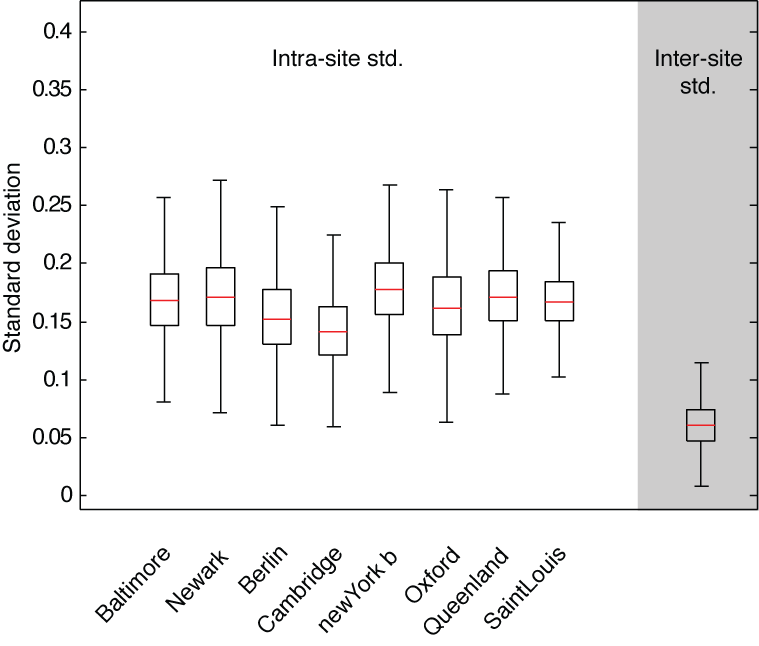
\includegraphics[width=\linewidth]{../figures/inter_vs_intra_3tonly.png}
\end{center}
\caption[inter vs. intra site variability]{
 Distribution of intra-site (between-subject) standard deviation vs. inter-site (between-site) standard deviation, based on the standard deviation of the connectivity matrices from a subset of 8 sites from the 1000 functional connectome dataset.
}
\label{fig_site_variability}
\end{figure}

\paragraph{Overall distribution across the connectome} Our first aim was to assess the amplitude of inter-site bias in resting-state connectivity measures. For each pair of parcels in the Cambridge functional atlas, and each pair of sites in the 1000 FCP, the absolute difference in connectivity, averaged across subjects, was derived between the two sites. The right boxplot in Figure \ref{fig_site_variability} shows the distribution (mean, std) of this inter-site measurement bias, across all possible connections and all possible pairs of sites. We observed that the amplitude of additive bias in group average connectivity measures was relatively small, with an average of about $0.05$. As a point of reference, the standard deviation (std) of functional connectivity measures was derived across all subjects. Figure \ref{fig_site_variability} shows the distribution (mean, std) of these intra-site std across all possible connections. The amplitude of intra-site std in connectivity across subjects was rather consistent across sites, with an average located in the 0.15 to 0.2 range. The amplitude of additive bias in group average connectivity measures was thus markedly smaller than the inter-subject, intra-site std (roughly 3-fold smaller, on the averages).


\begin{figure}[tbp]
\begin{center}
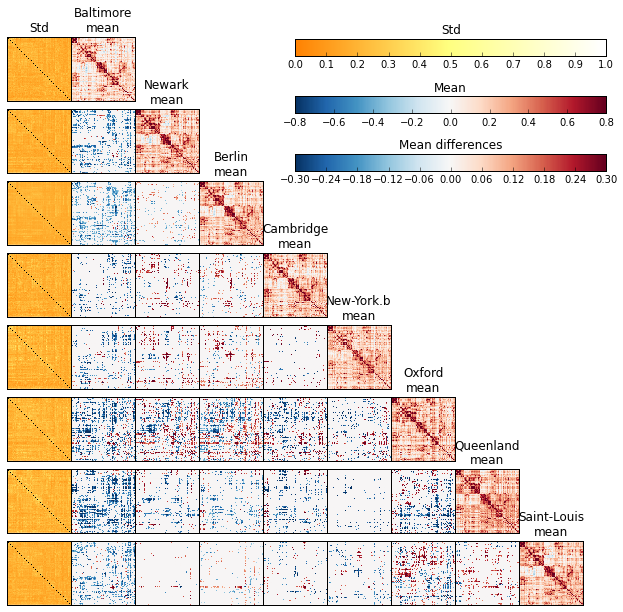
\includegraphics[width=\linewidth]{../figures/connectome_multisite.png}
\end{center}
\caption[Connectome variability across sites]{
Average functional connectome of 8 sites (Baltimore, Newark, Berlin, Cambridge, New-Yorkb, Oxford, Queenland and SaintLouis) are shown on the diagonal. The standard deviation across subjects and within site is shown on the first column. Each off-diagonal block represent the significant differences between the average functional connectome of two sites (called the inter-site bias). Statistical differences are obtained using a GLM procedure include age, sex and FD for each subject with an FDR correction procedure ($\alpha=0.05$).
}
\label{fig_connectome_variability}
\end{figure}

\paragraph{Connection-wise tests in the default-mode network} The distributions presented above agregated results across all possible brain connections in the Cambridge brain parcellation. To further clarify how the inter-site bias was distributed across connections, we first focused on the connections associated with a seed region located in the precuneus (PCC), a key node of the DMN \citep{Greicius2004}. The average connectivity map of the PCC was first extracted for each site, Figure \ref{fig_DMN_variability}. Qualitatively, the average PCC connectivity maps identified a network of regions consistent across sites and matching the distribution of the DMN, as reported in other studies \citep{Damoiseaux2006,Dansereau2014,Yan2013a}. At the intersection between two sites the difference in average connectivity is illustrated (red set of brain cuts). First The most salient changes between-sites are located in the mesio-frontal region associated with the anterior part of the DMN. In order to verify if significant changes are not only found in the DMN we have computed the entire connectome to obtain the other connectivity patterns and the findings can be generalized to the full connectome as illustraded in Figure \ref{fig_connectome_variability}.

\paragraph{Connectome-wide bias}
\begin{figure}[tbp]
\begin{center}
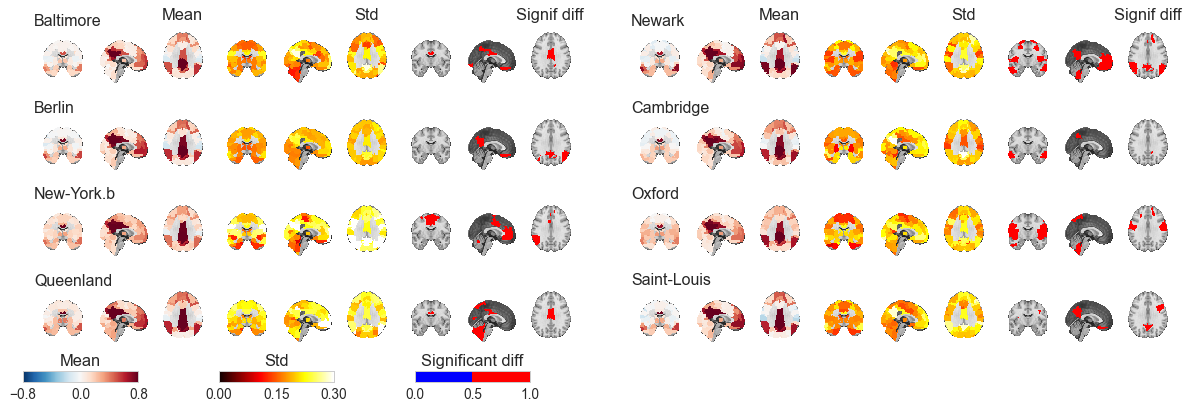
\includegraphics[width=\linewidth]{../figures/pccmap_multisite.png}
\end{center}
\caption[DMN variability across sites]{
Average functional connectivity maps of the default-mode network at on 8 sites (Baltimore, Newark, Berlin, Cambridge, New-Yorkb, Oxford, Queenland and SaintLouis). The average connectivity map are shown on the diagonal. The standard deviation across subjects and within site is shown on the first column. Each off-diagonal block represent the significant differences between the average functional connectivity maps of two sites (called the inter-site bias). Statistical differences are obtained using a GLM procedure include age, sex and FD for each subject with an FDR correction procedure ($\alpha=0.05$).
}
\label{fig_DMN_variability}
\end{figure}


\begin{figure}[tbp]
\begin{center}
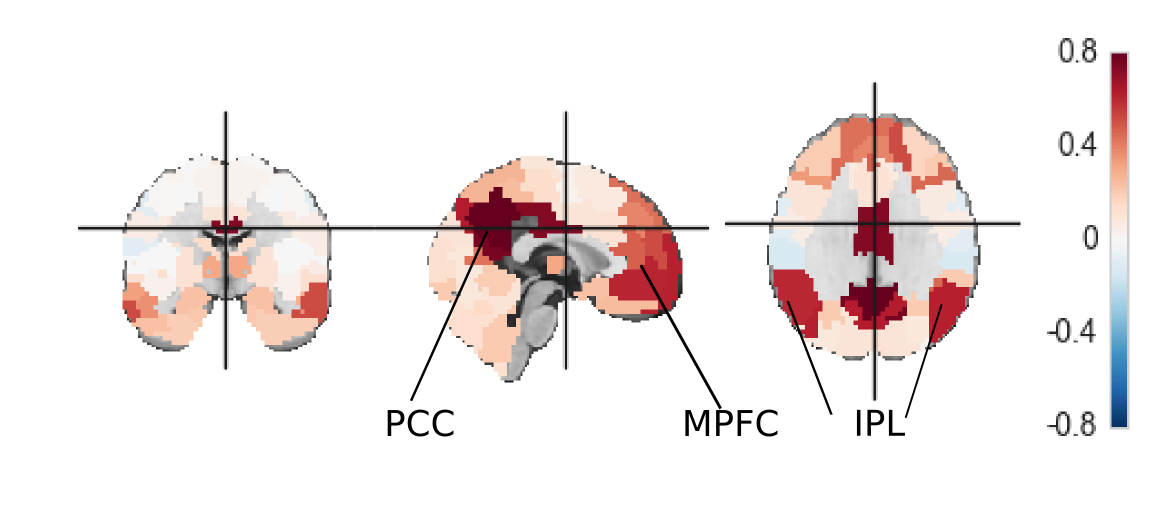
\includegraphics[width=0.7\linewidth]{../figures/dmn_reference.png}
\end{center}
\caption[]{
}
\label{fig_dmn_ref}
\end{figure}

\begin{figure}[tbp]
\begin{center}
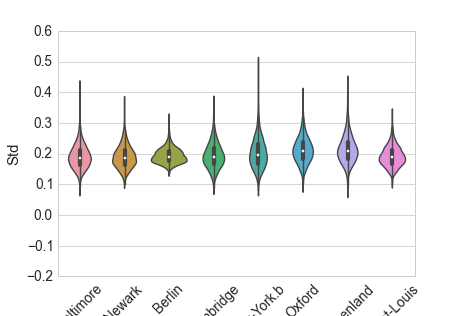
\includegraphics[width=0.7\linewidth]{../figures/boxplot_intrasite_var.png}
\end{center}
\caption[]{
}
\label{fig_dmn_ref}
\end{figure}


\begin{figure}[tbp]
\begin{center}
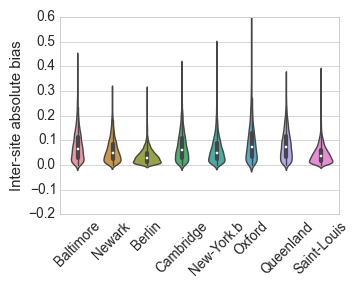
\includegraphics[width=0.7\linewidth]{../figures/boxplot_inter_var.png}
\end{center}
\caption[]{
}
\label{fig_dmn_ref}
\end{figure}

\begin{figure}[tbp]
\begin{center}
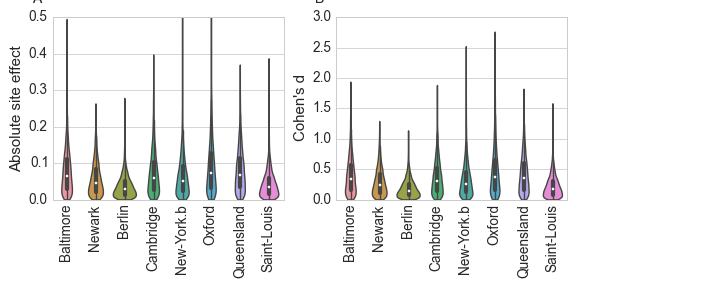
\includegraphics[width=0.7\linewidth]{../figures/boxplot_intra_inter_var.png}
\end{center}
\caption[]{
}
\label{fig_dmn_ref}
\end{figure}




\subsection{Simulation on real data}
In order to evaluate the impact of a multisite setup on our ability to detect changes in rs-functional connectivity studies we performed various simulation on real fMRI data. For each site and each sub-sample, $W$ of the subjects were randomly assigned to a 'treatment' group. For the subjects in this group, a value was added to achieve a given relative effect size expressed in Cohen's $d$. In order to detect changes on each connection pair between the artificially created groups, a general linear model (GLM) was applied and the following confounding variables were modelled in the analysis: age, sex and frame displacement (FD).

In Figure \ref{fig_real_sim} A) we show the effect of the sample size on the detection power. As expected we are able to detect smaller and smaller effect size as we increase the sample size. For an effect size of 1 which is considered a large effect we are able to detect significant changes in only 20\% of the cases at 40 subjects, 80\% at 80 subjects and almost 95\% at 120\% subjects.
Figure \ref{fig_real_sim} B) show the effect of debalancing the two groups at various allocation ratio $W$ (50\% , 30\% and 15\%) for a total sample-size of 120 subjects. Has the debalancing increase our ability to detect effect is diminished. As an example for an effect size of 1 we would detect the effect in 95\% of the cases in a 50 balanced scenario, this would go down to 90\% in a 30\%-70\% scenario and to 60\% in a 15\%-85\% scenario.
Figure \ref{fig_real_sim} C) show the effect of debalancing the two groups at various allocation ratio $W$ (50\% , 30\% and 15\%) with an interaction site-pathology (an effect of 0.5 Cohen's $d$ added to the model of half the sites) for a total sample size of 120 subjects. Has the allocation ratio is more debalanced our ability to detect effect is diminished. As an example for an effect size of 1 we would detect the effect in 98\% of the cases using a $W$ of 50\% scenario, this would go down to 95\% in a $W=$30\% scenario and to 75\% in a $W=$15\% scenario. The particularity of this experiment is the fact that the multisite configuration perform better than the single site meaning that it is better to have interaction of various amplitude across small sites than an average interaction on one large site.

\begin{figure}[tbp]
\centering
\captionsetup[subfloat]{labelformat=empty}
{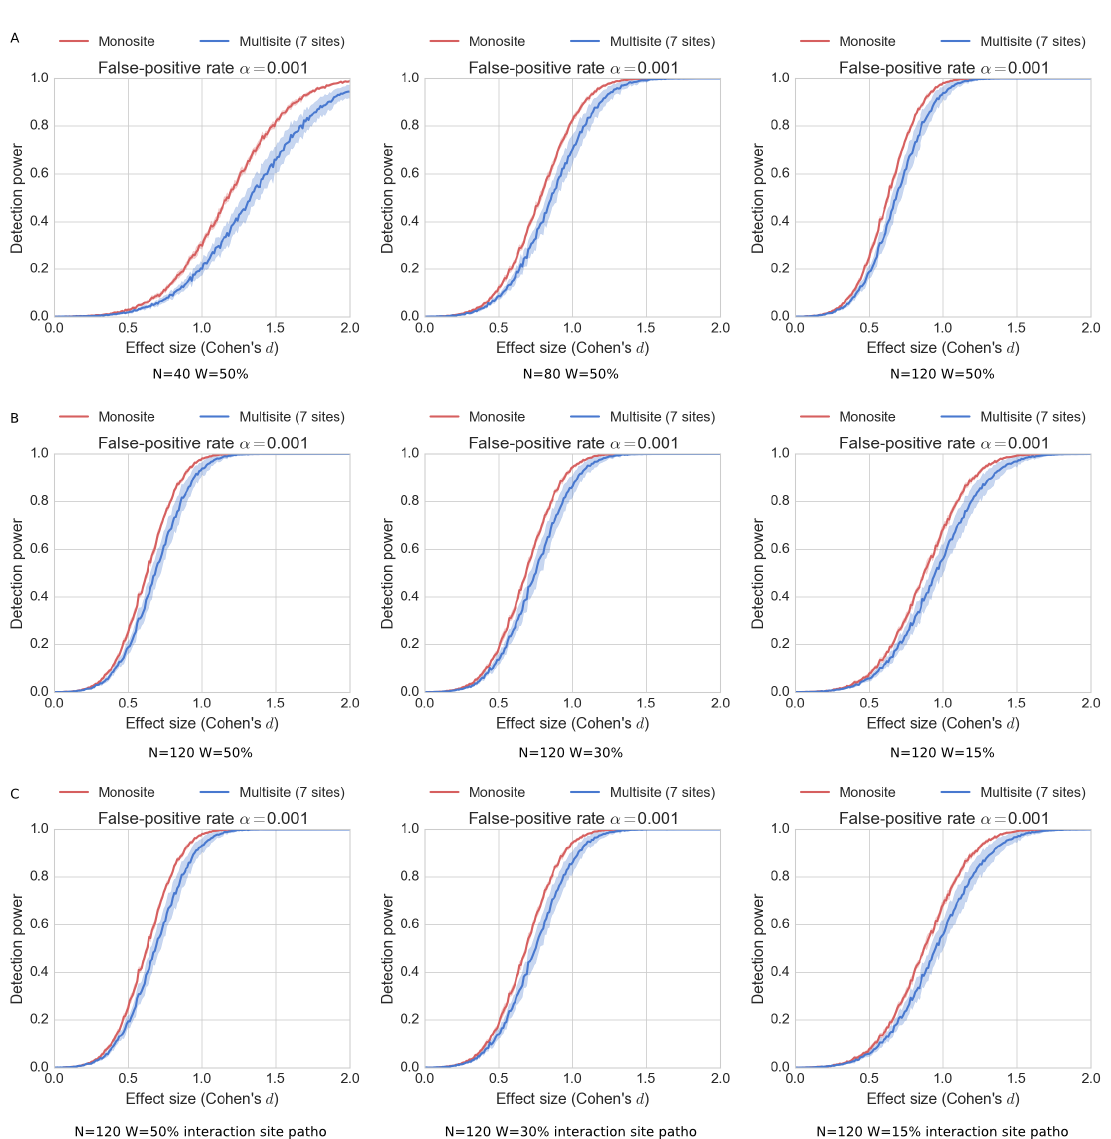
\includegraphics[width=\textwidth]{../figures/simulations_real_7sites.png}}

\caption{
A)Simulation on real data, detection power of two groups with an allocation ratio $W$ of 50\% between the 7 sites. Every plot show two scenarios: 1) monosite and 2) multisite 7 sites with correction for multisite differences using dummy variables. Each plot show the detection power in function of the effect-size for 3 different sample size 40, 80 and 120 subjects in total.
B)Simulation on real data, detection power of two groups for a total of 120 subjects between 7 sites. Every plot show two scenarios, 1) monosite and 2) multisite 7 sites with correction for multisite differences using dummy variables. Each plot show the detection power in function of the effect-size for 3 different allocation ratio $W$ of 50\%, 30\% and 15\% for each simulation.
C)Simulation on real data, detection power of two groups for a total of 120 subjects between 7 sites with a site-pathology interaction of  0.5 Cohen’s $d$. Every plot show two scenarios, 1) monosite and 2) multisite 7 sites with correction for multisite differences using dummy variables. Each plot show the detection power in function of the effect-size for 3 different allocation ratio $W$ of 50\%, 30\% and 15\% for each simulation.
}
\label{fig_real_sim}
\end{figure}



In Figure \ref{fig_sampeffect_curves_alpha001} show the sample-size in function of the effect-size for a detection power of 80\% using an allocation ratio $W$ of 50\%. A threshold on the statistical power of each test is applied at three alpha values: 0.001, (see alpha of 0.01 and 0.05 in supplementary material \ref{fig_sampeffect_curves_alpha01},\ref{fig_sampeffect_curves_alpha05}). We are reporting the parametric curve and the points obtained using our simulations for the monosite and the multisite. As we can see the monosite is concordant with the parametric estimation and the multisite is offset of approximately 20 subjects for the same effect-size. The variance in detection power across connections in multisite also diminish with larger sample-size and the difference between the parametric estimation and the monosite and multisite tend to vanish as we increase the sample size.

\begin{figure}[tbp]
\centering
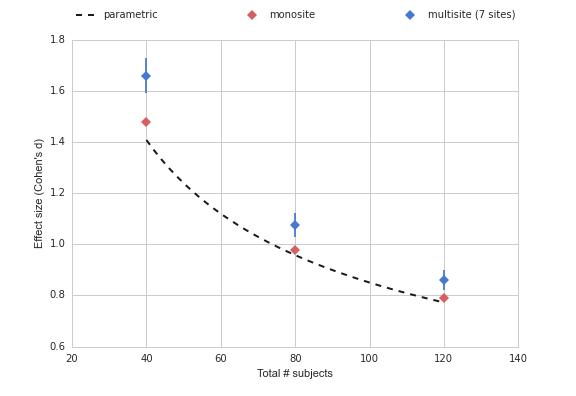
\includegraphics[width=0.65\textwidth]{../figures/samplesize_effectsize_pow80_alpha001.png}
\caption[]{
Sample-size in function of the effect-size for a detection power of 80\% using a threshold on the probability of having false-positive rate ($\alpha=0.001$) on a balanced dataset using an allocation ratio $W$ of 50\%.
}
\label{fig_sampeffect_curves_alpha001}
\end{figure}



Figure \ref{fig_real_sim_debalancing_2sites} show a scenario of two sites one large (80 subjects) and one small ($\sim20$ subjects) unbalanced at an allocation ratio $W$ of 30\% and the inverse ($W=$70\%) with an interaction site-pathology (an effect of 0.5 Cohen's $d$ added to the model of half the sites). As we can see the multisite configuration is as good as the monosite and the variance between connection is of the same order for the monosite and multisite.

\begin{figure}[tbp]
\centering
\captionsetup[subfloat]{labelformat=empty}
{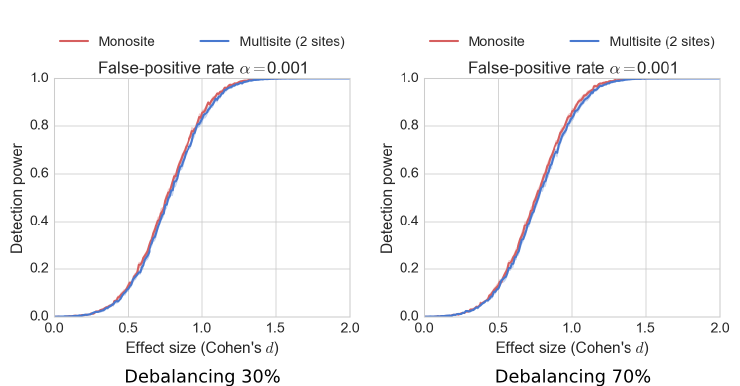
\includegraphics[width=.75\textwidth]{../figures/simulations_real_2sites.png}}

\caption{
Simulation on real data, detection power of two groups for a total of 100 subjects between 2 sites with a site-pathology interaction of  0.5 Cohen’s $d$, one small site of 20 subjects and one large of 80 subjects. Every plot show two scenarios, 1) monosite and 2) multisite 2 sites with correction for multisite differences using dummy variables. Each plot show the detection power in function of the effect-size for 2 different allocation ratio $W$ of 30\% and 70\% between 2 sites.
}
\label{fig_real_sim_debalancing_2sites}
\end{figure}


Using these Monte-Carlo simulations we have shown that the power of detecting an effect is marginally affected by the site acquisition configuration (monosite or multisite) when the sites are balanced in term of the amount of subject.


%%%%%%%%%%%%%%%%%%%%%%%%%%%%%%%%%%%%%%%%%%%%%
% END of results section                    %
%%%%%%%%%%%%%%%%%%%%%%%%%%%%%%%%%%%%%%%%%%%%%

\section{Discussion}

An important benefit of multisite acquisitions is to offer improved generalization compared to single site studies, due to more diversity in scanners and populations. These additional sources of variance may however decrease the statistical power, and somewhat mitigate the benefits of having a large sample size. In this work, our main objective was to quantitatively assess the impact of inter-site variability on statistical power, for rs-fMRI group comparison.


To establish the impact of multisite acquisitions on statistical power in rs-fMRI, we first specifically aimed at characterizing the amplitude of the inter-site bias in real rs-fMRI measures, relative to intra-site variance. We based our evaluation on N=345 young healthy participants from the 1000 Functional Connectomes Project (FCP), including rs-fMRI samples independently collected at 8 imaging sites with 3T scanners in Germany, the United Kingdom, Australia and the United States of America. Datasets in this study were shared retrospectively and every documented parameters of image acquisition varied across studies. This data sample thus represents a worst-case-scenario in terms of 3T instrumental inter-site variations. Our second specific aim was to evaluate the impact of such inter-site bias on the detection power of rs-fMRI group comparison, in relation with sample size, group balancing and interaction between sites and group differences. We implemented for this purpose a series of simulation, mixing synthetic data with real data from the 1000 FCP. One of the particularity of the 1000 FCP is the presence of one large site of $\sim200$ subjects and 7 small sites of $\sim20$ subjects per site. We were therefore able to implement realistic scenarios following either a monosite or a multisite design, with the same total sample size.

This work therefore confirm the existence of an inter-site connectivity bias and compared it to the intra-site bias.\\
The contribution of the intra and inter-subject variability is about 3 fold greater than the inter-site contribution.\\
 
Connectivity bias can impact interpretation.\\

In this study the great majority of scanner were Siemens,and therefore more variability may be found using various brands unfortunatly this avenue was not testable in using this dataset.\\


Talk about the impact in small acquisition 40 subjects total and the importance of pooling data among PI.\\
Choosing the right sample size for a given detection power to obtain reproducible results.

Talk about the impact in clinical trial and best practice.\\
	most of the time we cannot correct for site with one population only or with too few subjects per site. Although these kind of multisite studies generally sum-up to large dataset of more than 200 subjects. has we demonstrated in the synthetic simulation such configuration are comparable to single site analysis for this range of sample size.

It is better to have interaction of various amplitude across small sites than an average interaction on one large site\\

The number of subject / site will impact the bias between multisite and monosite (like in the example of 2 sites the diff is marginal). Resulting in the following conclusion combining large site (e.g greater than 50 subjects) may results in low bias compared to very small sites.

talk about the reduction of the bias of the simulation compared to the fully parametric estimate as we increase the sample size. The estimation is more realistic over 80 subjects and overestimate the detection power at low sample-size.

% can be use for other multisite study...
Despite justifiable scepticism, feasibility analyses demonstrated that meaningful explorations of the aggregate dataset, composed of 24 imaging sites for a grand total of 1093 subjects, could be performed \citep{Biswal2010}. Although no explicit correction for multi-site variability was used, they only use global signal correction (GSC) to normalize subjects which may introduce anti-correlation in the data \citep{Fox2009, Murphy2009, Saad2012, Carbonell2014, Power2014}. After accounting for site-related differences, the analysis showed brain-behaviour relationships with phenotypic variables such as age, gender, and diagnostic label, and confirmed a variety of prior hypotheses \citep{Biswal2010, Fair2012, Tomasi2010, Zuo2012}. While encouraging, many uncontrolled and unknown factors in the 1000 FCP remain a source of concern, as they spread beyond simple site effects and can limit the datasets utility as highlighted by \cite{Yan2013}. Another compelling proof of multisite bias is the study reported by \cite{Nielsen2013} where they did an analysis on a single site dataset and a multi-site dataset of subject with autism and concluded that the multi-site autism study classification accuracy significantly outperformed chance but was much lower for multi-site prediction than for previous single site results \citep{Nielsen2013}. We therefore need to keep in mind that the site effect must be taken in account in the analysis or we may reduce our detection power.

\section{Conclusion}


\section{Acknowledgments}
Parts of this work were presented at the 2013 annual meetings of the organization for human brain mapping \citep{Dansereau2013a}, as well as the  Alzheimer's Association International Conference (AAIC) (2013) (Boston) \citep{Dansereau2013b}. The authors are grateful to the members of the 1000 functional connectome consortium for publicly releasing there dataset. The computational resources used to perform the data analysis were provided by ComputeCanada\footnote{\url{https://computecanada.org/}} and CLUMEQ\footnote{\url{http://www.clumeq.mcgill.ca/}}, which is funded in part by NSERC (MRS), FQRNT, and McGill University. This project was funded by NSERC grant number RN000028, a salary award from ``Fonds de recherche du Qu\'ebec -- Sant\'e'' to PB as well as a salary award by the Canadian Institute of Health Research to CD.

\section*{References}

\bibliographystyle{elsarticle-harv}
\bibliography{cdansereau}


\pagebreak



\clearpage
\appendix


%% SUPPLEMENTARY MATERIAL
\clearpage
\pagebreak
\renewcommand{\thefigure}{S\arabic{figure}}
\renewcommand{\thetable}{S\arabic{table}}
\setcounter{figure}{0}
\begin{center}
\emph{Supplementary Material {--} Feasibility of multi-centric fMRI connectivity studies of Alzheimer's disease}\\

\vspace{\baselineskip}Submitted to Neuroimage.\\

\vspace{\baselineskip}C. Dansereau$^{1,2}$,  C. Risterucci$^{3}$, E. Merlo Pich$^{3}$, D. Arnold$^{4}$, P. Bellec$^{1,2}$\\

\end{center}
$^1$Functional Neuroimaging Unit, Centre de Recherche de l'Institut Universitaire de G\'eriatrie de Montr\'eal\\
$^2$Department of Computer Science and Operations Research, University of Montreal, Montreal, Quebec, Canada\\
$^3$F. Hoffmann-La Roche Ldt., Basel, Switzerland\\
$^4$NeuroRx, Montreal, Quebec, Canada\\

For all questions regarding the paper, please address correspondence to Pierre Bellec, CRIUGM, 4545 Queen Mary, Montreal, QC, H3W 1W5, Canada. Email: pierre.bellec (at) criugm.qc.ca.\\

\section*{Supplementary Material} 

\begin{figure}[tbp]
\centering
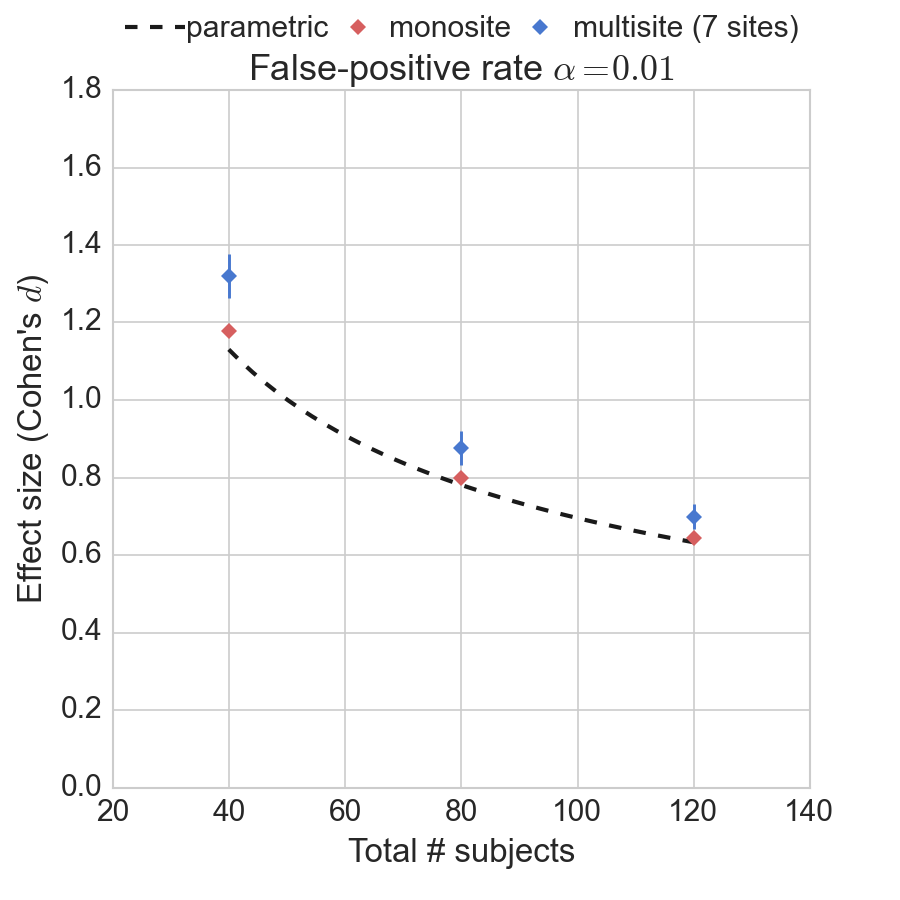
\includegraphics[width=0.50\textwidth]{../figures/samplesize_effectsize_pow80_alpha01.png}
\caption[]{
Sample-size in function of the effect-size for a detection power of 80\% using a threshold on the probability of having false-positive rate ($\alpha=0.01$) on a balanced dataset using an allocation ratio $W$ of 50\%.
}
\label{fig_sampeffect_curves_alpha01}
\end{figure}
\begin{figure}[tbp]
\centering
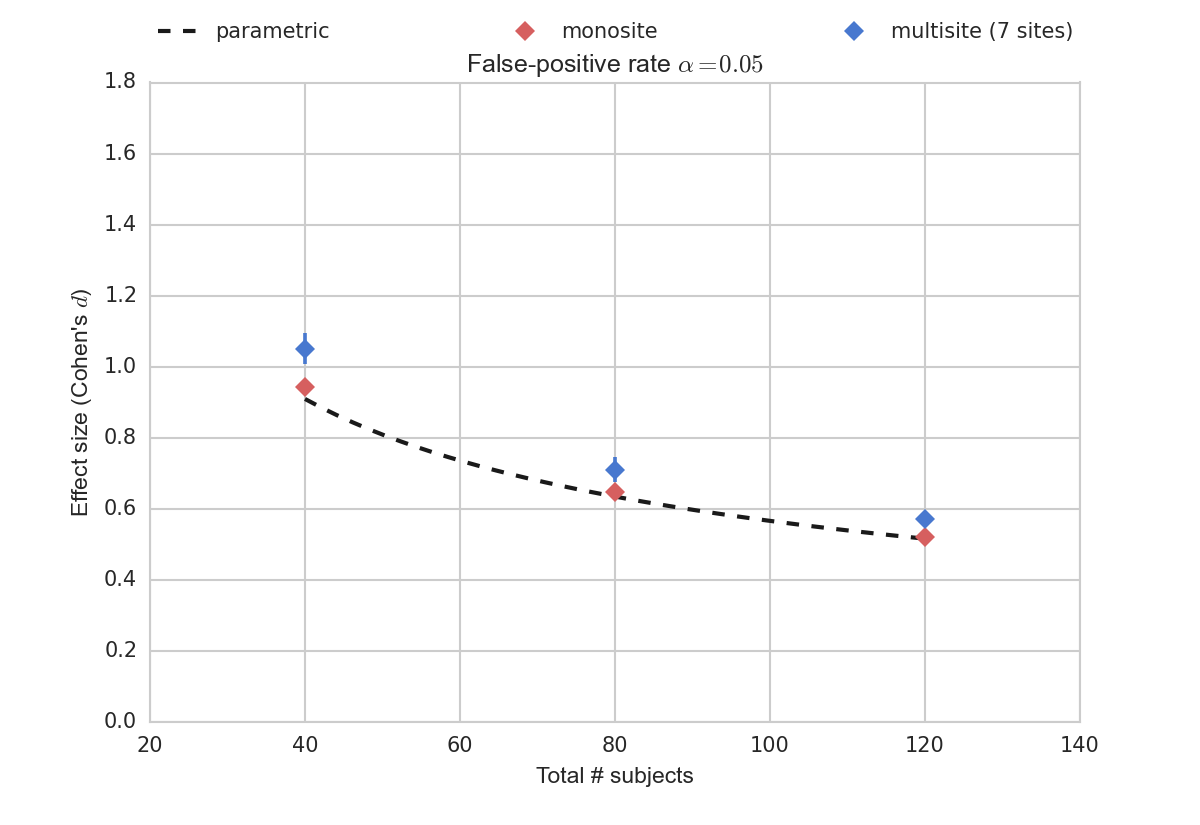
\includegraphics[width=0.50\textwidth]{../figures/samplesize_effectsize_pow80_alpha05.png}
\caption[]{
Sample-size in function of the effect-size for a detection power of 80\% using a threshold on the probability of having false-positive rate ($\alpha=0.05$) on a balanced dataset using an allocation ratio $W$ of 50\%.
}
\label{fig_sampeffect_curves_alpha05}
\end{figure}

\end{document}


